\chapter{Testing Progress}

\section{Backend Tested}

\subsection{Coverage}
% Insert backend coverage image here
\begin{center}
    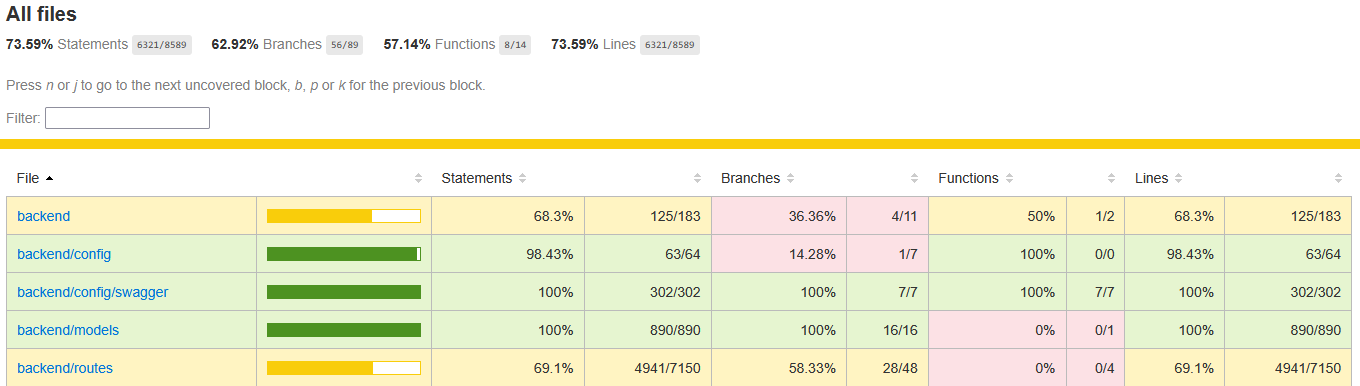
\includegraphics[width=0.8\textwidth]{cov/backend-coverage.png}
\end{center}

\subsection{Test Cases}
\begin{itemize}
    \item[\textbf{\checkmark}] \textbf{Test-Api-Info}
    \begin{itemize}
        \item \textbf{Description:} Information about our Api shows.
        \item \textbf{Reason:} To easily check if our Api is up.
    \end{itemize}
    
    \item[\textbf{\checkmark}] \textbf{Test-Public-Course-Get-Endpoint}
    \begin{itemize}
        \item \textbf{Description:} Get the all courses from public endpoint.
        \item \textbf{Reason:} Have public endpoint for external use.
    \end{itemize}
    
    \item[\textbf{\checkmark}] \textbf{Test-Private-Course-Get-Endpoint}
    \begin{itemize}
        \item \textbf{Description:} Get the all courses from private endpoint.
        \item \textbf{Reason:} Have private endpoint for getting courses.
    \end{itemize}
    
    \item[\textbf{\checkmark}] \textbf{Test-Private-Resources-Get-Endpoint}
    \begin{itemize}
        \item \textbf{Description:} Get the all resources from private endpoint.
        \item \textbf{Reason:} Have private endpoint for getting resources or specific resource.
    \end{itemize}
    
    \item[\textbf{\checkmark}] \textbf{Test-User-Get-Endpoint}
    \begin{itemize}
        \item \textbf{Description:} Check if we can get users by Id or All.
        \item \textbf{Reason:} To get all users or specific users.
    \end{itemize}
    
    \item[\textbf{\checkmark}] \textbf{Test-User-Get-notification}
    \begin{itemize}
        \item \textbf{Description:} Check if we can get users by Id or All.
        \item \textbf{Reason:} To get all users or specific users.
    \end{itemize}
    
    \item[\textbf{\sout{\ \ }}] \textbf{Authentication}
    \begin{itemize}
        \item \textbf{Description:} Testing the authentication endpoint directly.
        \item \textbf{Reason:} The test is not done because it is indirectly tested via login functionality
    \end{itemize}
\end{itemize}

\section{Frontend Tested}

\subsection{Coverage}
% Insert frontend coverage image here
\begin{center}
    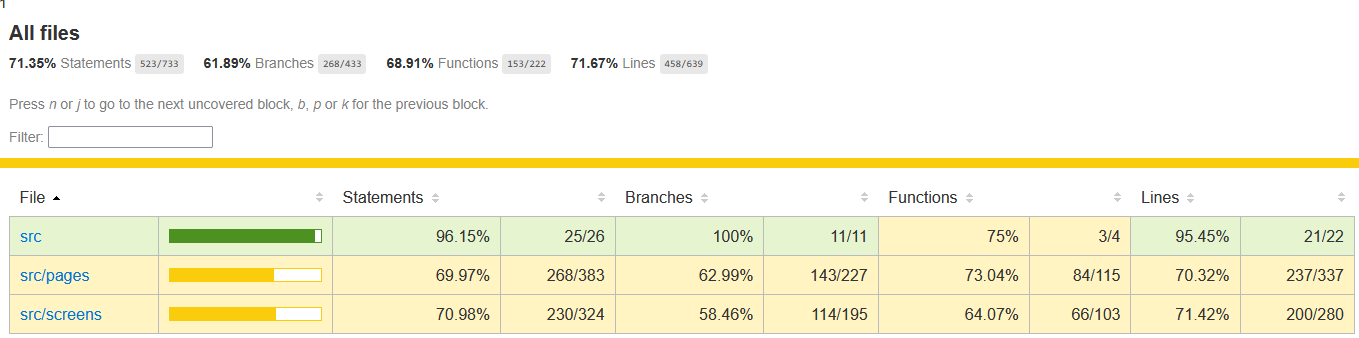
\includegraphics[width=0.8\textwidth]{cov/frontend-coverage.png}
\end{center}

\subsection{Test Cases}
\begin{itemize}
    \item[\textbf{\checkmark}] \textbf{Test-Login}
    \begin{itemize}
        \item \textbf{Description:} Test if user can correctly with Google email.
        \item \textbf{Reason:} If user cannot login they cannot use the app.
    \end{itemize}
    
    \item[\textbf{\checkmark}] \textbf{Test-Saving-State}
    \begin{itemize}
        \item \textbf{Description:} Saving the Login state for all tests to use
        \item \textbf{Reason:} To avoid being block for automated testing by Google.
    \end{itemize}
\end{itemize}

\section{Issues}

\subsection{npm Packages 2025-09-21}
\begin{itemize}
    \item 180 packages are looking for funding
    \item Run \texttt{npm fund} for details
    \item 1 low severity vulnerability
    \item To address all issues, run: \texttt{npm audit fix}
    \item Run \texttt{npm audit} for details
\end{itemize}

\subsection{Env Files Being Tracked Fix}
\begin{verbatim}
git rm --cached frontend/.env
git rm --cached frontend/.env.*
git rm --cached backend/.env
git rm --cached backend/.env.*
git commit -m "Stop tracking .env files in frontend and backend"
\end{verbatim}

\section{Package Audit Report}

\subsection{Audit Details}
\begin{itemize}
    \item \textbf{Audit Date:} 2025-09-30T13:54:43.105518
\end{itemize}

\subsection{Frontend Audit}
\begin{itemize}
    \item \textbf{Total Packages:} 584
    \item \textbf{Compromised:} 21
    \item \textbf{Compromised Percentage:} 3.6\%
    \item \textbf{Safe Percentage:} 96.4\%
\end{itemize}

\textbf{Compromised Packages:}
\begin{verbatim}
- ansi-regex@6.2.2
- ansi-styles@6.2.3
- strip-ansi@7.1.2
- wrap-ansi@8.1.0
- debug@4.1.12
- ansi-regex@5.0.1
- ansi-styles@4.3.0
- chalk@4.1.2
- color-convert@2.0.1
- color-name@1.1.4
- debug@4.4.1
- debug@4.3.7
- debug@4.3.7
- debug@1.0.0
- debug@4.3.7
- debug@4.3.7
- debug@4.3.7
- debug@4.3.7
- strip-ansi@6.0.1
- supports-color@7.2.0
- wrap-ansi@6.2.0
\end{verbatim}

\subsection{Backend Audit}
\begin{itemize}
    \item \textbf{Total Packages:} 1043
    \item \textbf{Compromised:} 34
    \item \textbf{Compromised Percentage:} 3.26\%
    \item \textbf{Safe Percentage:} 96.74\%
\end{itemize}

\textbf{Compromised Packages:}
\begin{verbatim}
- ansi-regex@6.2.2
- ansi-styles@6.2.3
- strip-ansi@7.1.2
- wrap-ansi@8.1.0
- debug@4.1.12
- ansi-regex@5.0.1
- ansi-styles@4.3.0
- debug@2.6.9
- chalk@4.1.2
- color-convert@2.0.1
- color-name@1.1.4
- debug@2.6.9
- debug@4.4.3
- debug@4.3.7
- debug@4.3.7
- error-ex@1.3.4
- debug@3.2.7
- debug@3.2.7
- debug@3.2.7
- debug@2.6.9
- debug@2.6.9
- is-arrayish@0.2.1
- supports-color@8.1.1
- debug@2.6.9
- supports-color@5.5.0
- ansi-styles@5.2.0
- debug@2.6.9
- debug@4.3.7
- debug@4.3.7
- debug@4.3.7
- debug@4.3.7
- strip-ansi@6.0.1
- supports-color@7.2.0
- wrap-ansi@7.0.0
\end{verbatim}

\subsection{Overall Summary}
\begin{itemize}
    \item \textbf{Total Packages:} 1627
    \item \textbf{Total Compromised:} 55
    \item \textbf{Overall Compromised:} 3.38\%
    \item \textbf{Overall Safe:} 96.62\%
\end{itemize}

\textbf{Assessment:} The low compromise rate (3.38\%) reflects minimal security concerns, as these vulnerabilities originate from external package dependencies rather than our core application code, presenting acceptable risk levels for our current deployment. Hance no action is required.

